\documentclass[../Relazione.tex]{subfiles}

\begin{document}
\section{Conclusioni}
    Abbiamo analizzato i valori medi (in rif. alla tabella \#\ref{fig:tot_avg}) in relazione al costo aggiuntivo che comporterebbe ogni assunzione (\euro400) ed abbiamo realizzato un grafico che riassume le nostre analisi.
    \vspace{0.5cm}
    \begin{figure}[!h]
        \centering
        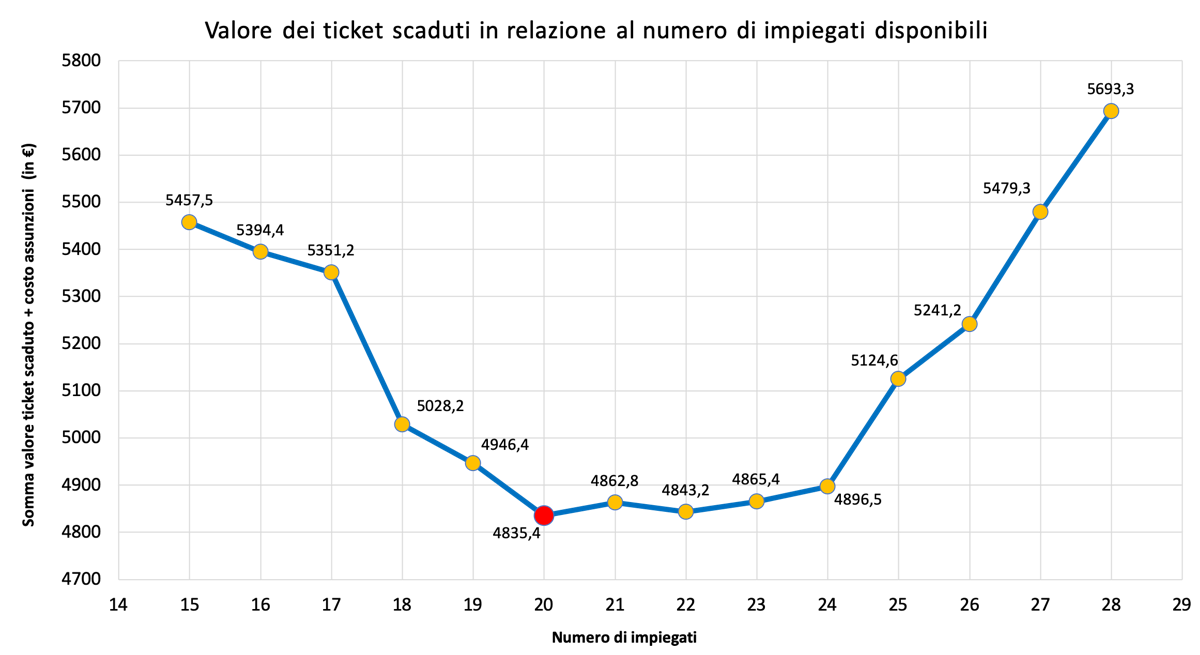
\includegraphics[scale=0.8]{ATCS/figures/plot_analysis.png}
        %\caption{Caption}
        \label{fig:plot_anal}
    \end{figure}
    
    Come si può evincere da tale grafico, il guadagno maggiore (ovvero il valore minore dell'ammontare totale dei ticket scaduti più il costo delle nuove assunzioni) si ottiene con \textbf{20 impiegati}. Il valore riportato (\euro4835.4) è minore anche del valore calcolato senza assumere nessun nuovo impiegato (\euro5457.5) e questo, quindi, \textbf{giustifica l'assunzione di 5 nuovi impiegati}.
         
\end{document} 
		